\section{Alternatives exploration}
\label{Implementation:Alternatives}

The Massive Online Analysis stream mining framework is built in the Java language, thus providing some benefits in terms of portability, ease of maintenance and development, but also exposing some drawbacks, mainly due to the lack of easily parallelizable code, like is the case with C or Fortran by using the OpenMP\footnote{OpenMP (Open Multi-Processing) is a programming interface that supports multi-platform shared memory multiprocessing programming in C, C++, and Fortran. It consists of a set of compiler directives, library routines, and environment variables that influence run-time behavior.~\citep{web:Wiki:OpenMP}} language extensions. Given the language enforcement MOA imposes and the existence of well-known SDC toolsuites, like the \texttt{sdcMicro} R package (reviewed in~\sref{State::SDC::sdcMicro}), an analysis of possible alternatives was taken during the first weeks of the project's development phase.

\subsection{\texttt{sdcMicro} \& Java}
\label{Implementation:Alternatives:sdcmicro}

The most direct alternative, besides actually implementing the filters, was to use the \texttt{sdcMicro} library to perform the necessary calculations over the streaming data originated in MOA and take the results back to the framework. This approach can be better understood in~\fref{fig:ppsm-R}: a bi-directional connection between the Java runtime (the Java Virtual Machine or JVM) and the R process would be needed to be able to use the SDC methods of the \texttt{sdcMicro} library. The results of the exploratory analysis of this type of solution are summarized in~\tref{table:JRI-pros-cons}.

\begin{figure}[h]
	\centering
	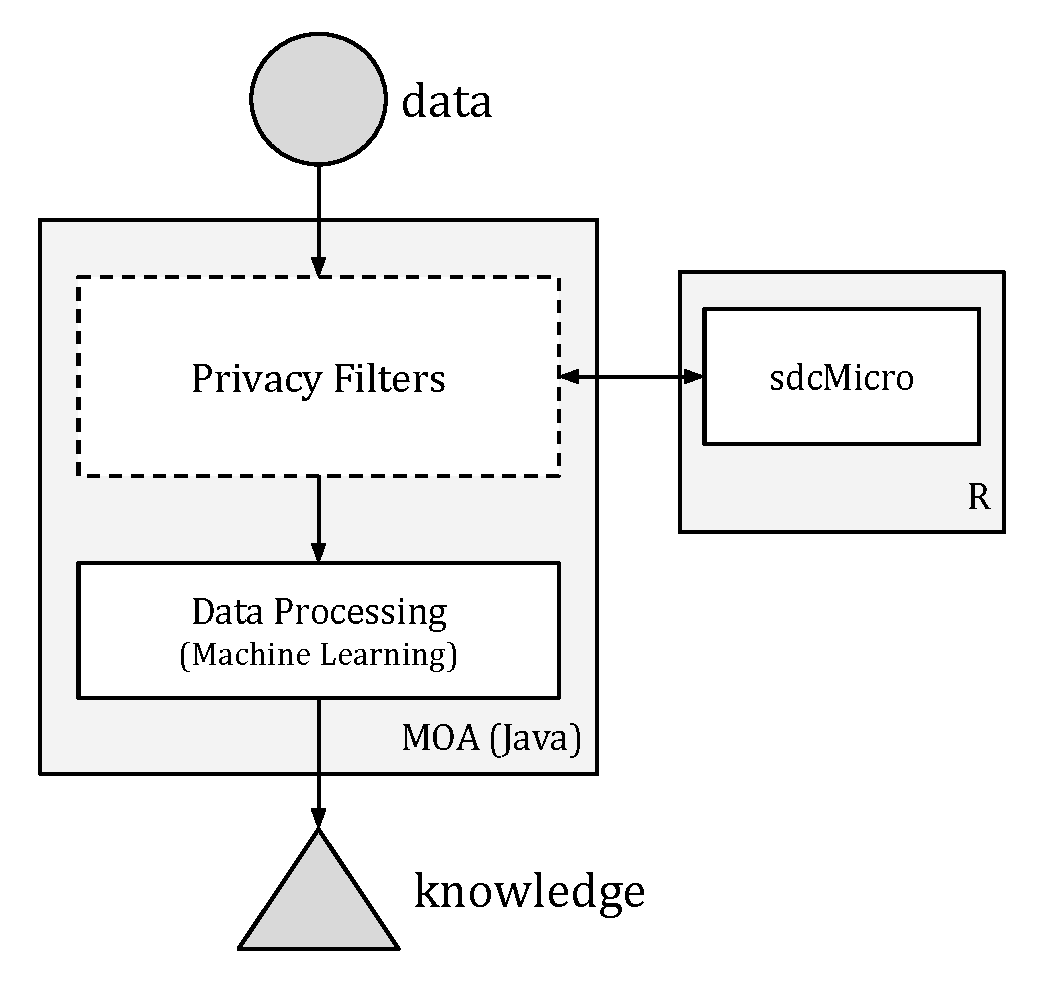
\includegraphics[width=0.6\textwidth]{figures/moa-ppsm-R.pdf}
	\caption{R/Java hybrid solution using the \texttt{sdcMicro} package.}
	\label{fig:ppsm-R}
\end{figure}

This interconnection could be achieved by using some existing technologies that perform the inter-process communication based on different approaches:

\begin{itemize}
	\item
	\textbf{rJava/JRI:} the \texttt{rJava} and \texttt{JRI} counterparts are a couple of libraries designed to provide low-level communication between the Java Virtual Machine (JVM) and an R process. \texttt{rJava} provides a low-level bridge between R and Java via the Java Native Interface (JNI)\footnote{The Java Native Interface is a standard programming interface for writing Java native methods and embedding the Java Virtual Machine into native applications. The primary goal is binary compatibility of native method libraries across all Java virtual machine implementations on a given platform~\citep{web:Oracle:JNI}.}. It allows to create objects, call methods and access fields of Java objects from R~\citep{web:rJava}. On the other side, \texttt{JRI} is a Java/R Interface, which allows to run R inside Java applications as a single thread. Basically, it loads R dynamic library into Java and provides a Java API to R functionality~\citep{web:JRI}.
	
	\item
	\textbf{Rserve:} it is a TCP/IP server which allows other programs to use facilities of R from various languages without the need to initialize R or link against an R library. A typical use is to integrate R backend for computation of statstical models, plots etc. in other applications~\citep{web:Rserve}.
\end{itemize}

Due to performance related to networking protocols against native interface communication, \texttt{Rserve} was discarded as an option to implement filters for MOA: a streaming environment requires the maximum throughput possible for its algorithms and, thus, the overhead associated with TCP-based IPC is considered to be excessive.

Anyway, either of such solutions imply that marshalling and unmarshalling techniques would have to be applied, in order to transform the data structures that are differently used by R and Java. Moreover, even though that no SDC algorithm would need to be implemented, the interconnect code would not be easy to maintain.

Finally, there is another important argument against the R/Java hybrid approach: its strong reliance in external dependencies. These dependencies not only make the installation of the SDC-enabled MOA framework more difficult, but are directly linked to third-party software and \textit{system} libraries, making the environment less stable and robust, from the software user point of view. These dependencies are shown in~\fref{fig:ppsm-JRI-arch}

\begin{figure}[h]
	\centering
	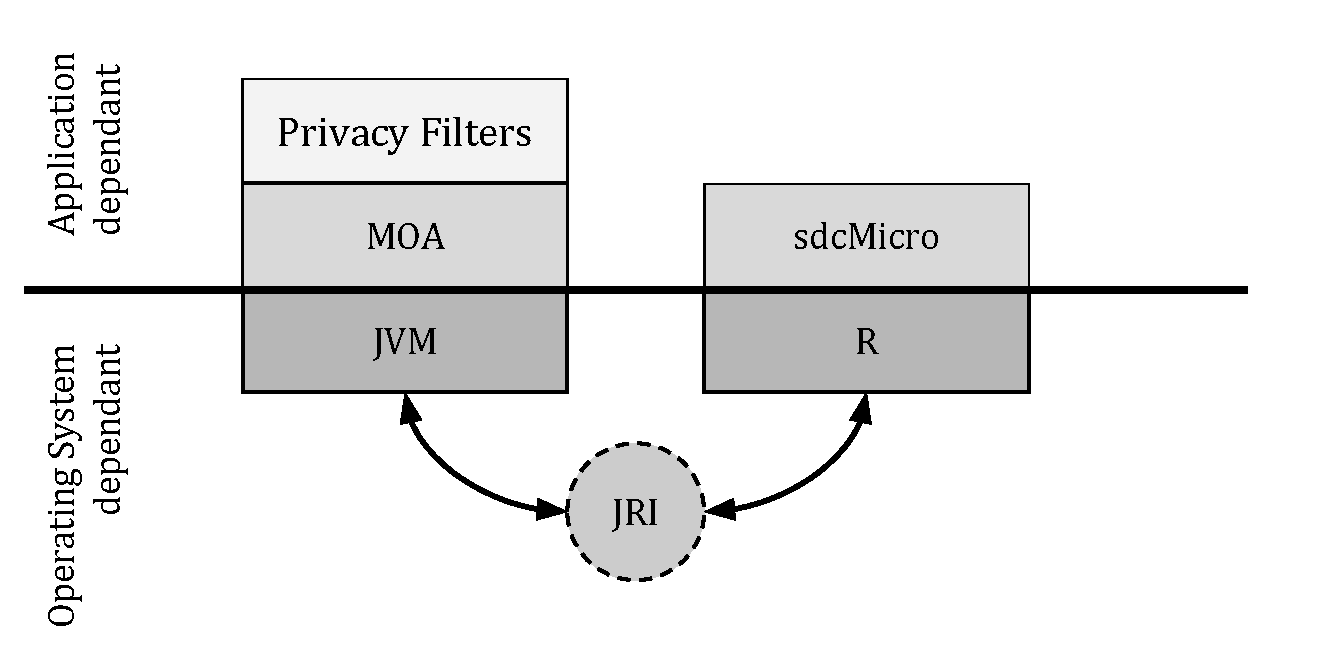
\includegraphics[width=0.8\textwidth]{figures/moa-ppsm-JRI-arch.pdf}
	\caption{JRI based R/Java hybrid solution architechture: strong dependencies.}
	\label{fig:ppsm-JRI-arch}
\end{figure}

\begin{table}
	\centering
	\begin{tabular}{ll}
		\hline
		\textbf{Benefits}     & \textbf{Drawbacks}                     \\ \hline
		Faster development    & No algorithms are indeed developed     \\
		Easily extensible     & Strong dependencies                    \\
		SDC methods are right & Depends on external installed software \\
		                      & Needs system libraries to work         \\
		                      & Maintanability is harder               \\
		                      & Reduced performance due to marshalling \\ \hline
	\end{tabular}
	\caption{Evaluation of the R/Java hybrid solution.}
	\label{table:JRI-pros-cons}
\end{table}

\subsubsection{Renjin}

Yet another altenative was explored that was meant to interconnect MOA with the \texttt{sdcMicro} package: the Renjin project~\citep{web:Renjin}. \textbf{Renjin} is a JVM-based interpreter for the R language: all computations of any R package can be executed upon the JVM, instead of a separate R process. This way, the dependency that this project could have had on R and some system libraries disappeared. However, it is worth noting that, even with Renjin, data structures conversion would have to be performed, rendering its use as impractical as the use of the \texttt{JRI} library. Moreover, the \texttt{sdcMicro} package was still not available in its JVM \textit{port} at the time of the evaluation due to some internal dependencies and errors, and we could not wait for it to be solved.

\subsection{Chosen alternative}

As a simple remark, the final decision was to actually develop the filters for the MOA framework by extending it, in the form of a \textbf{pure Java} implementation.